\documentclass[12pt]{article}
\usepackage{cwilliams-standard}

\setclass{\MLONE}
\settitle{Homework 6 \\ \Large{Simply \& Multiple Linear Regression Analysis}}

\begin{document}

\maketitlepage

\begin{important}{Console Outputs}
    For every question that requires an output in the console of the program, the output will be seen in the program,
    but I will also include answers in this document for easier grading (I hope). Thank you for your hard work!
\end{important}

\section{EDA}

\subsection{Shelve Location vs Sales Analysis}

\begin{figure}[H]
    \centering
    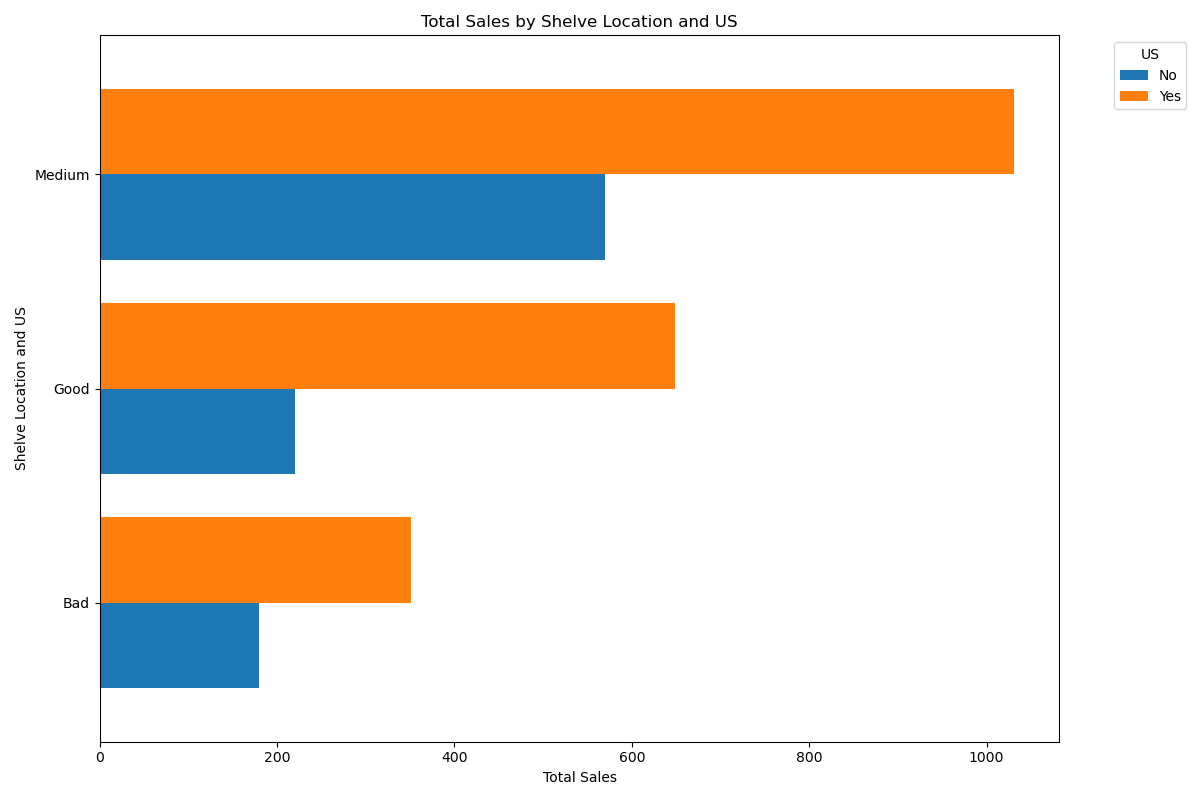
\includegraphics[width=0.9\textwidth]{images/sales_by_shelveloc_us.png}
    \caption{ShelveLoc vs Sales grouped by US location}
    \label{fig:shelveloc_sales}
\end{figure}

\subsection{One-Hot Encoding}

The dataset was successfully encoded using one-hot encoding. The qualitative features (ShelveLoc, Urban, US) were converted to binary features while avoiding the dummy trap by dropping one category from each.


\subsection{Train-Test Split and Standardization}

The dataset was split with 80\% training (320 samples) and 20\% testing (80 samples) with shuffle=True and random\_state=5805. The continuous features were standardized while encoded features were kept binary.


Then, for ease of use later in on in the file, I kept the \textbf{Sales scaling parameters} so that reverse transforms would be easier.
\textbf{Sales scaling parameters:}
\begin{itemize}
    \item Mean: 7.5120
    \item Scale (std): 2.8262
\end{itemize}

\section*{Feature Selection \& Prediction}

\section{Backward Stepwise Regression}

\subsection{Elimination Process Table}

The backward stepwise regression started with 11 features and eliminated 4 features based on p-value threshold of 0.01.
\begin{table}[H]
\centering
\caption{Backward Stepwise Regression Elimination Process}
\begin{tabular}{ccccccc}
\toprule
\textbf{Iteration} & \textbf{Features Count} & \textbf{Feature Eliminated} & \textbf{P-value} & \textbf{AIC} & \textbf{BIC} & \textbf{Adj. $R^2$} \\
\midrule
1 & 11 & Population & 0.962 & -633.132 & -587.913 & 0.867 \\
2 & 10 & Education & 0.599 & -635.130 & -593.679 & 0.867 \\
3 & 9 & US\_Yes & 0.338 & -636.843 & -599.160 & 0.867 \\
4 & 8 & Urban\_Yes & 0.213 & -637.893 & -603.978 & 0.867 \\
5 & 7 & None & - & -638.298 & -608.151 & 0.867 \\
\bottomrule
\end{tabular}
\end{table}

\textbf{Eliminated Features (4):}
\begin{enumerate}
    \item Population (p-value: 0.962)
    \item Education (p-value: 0.599)
    \item US\_Yes (p-value: 0.338)
    \item Urban\_Yes (p-value: 0.213)
\end{enumerate}

\textbf{Final Selected Features (7):}
\begin{enumerate}
    \item CompPrice
    \item Income
    \item Advertising
    \item Price
    \item Age
    \item ShelveLoc\_Good
    \item ShelveLoc\_Medium
\end{enumerate}

\subsection{OLS Regression Summary}

Five OLS regression summaries are provided showing the elimination process:

\begin{figure}[H]
    \centering
    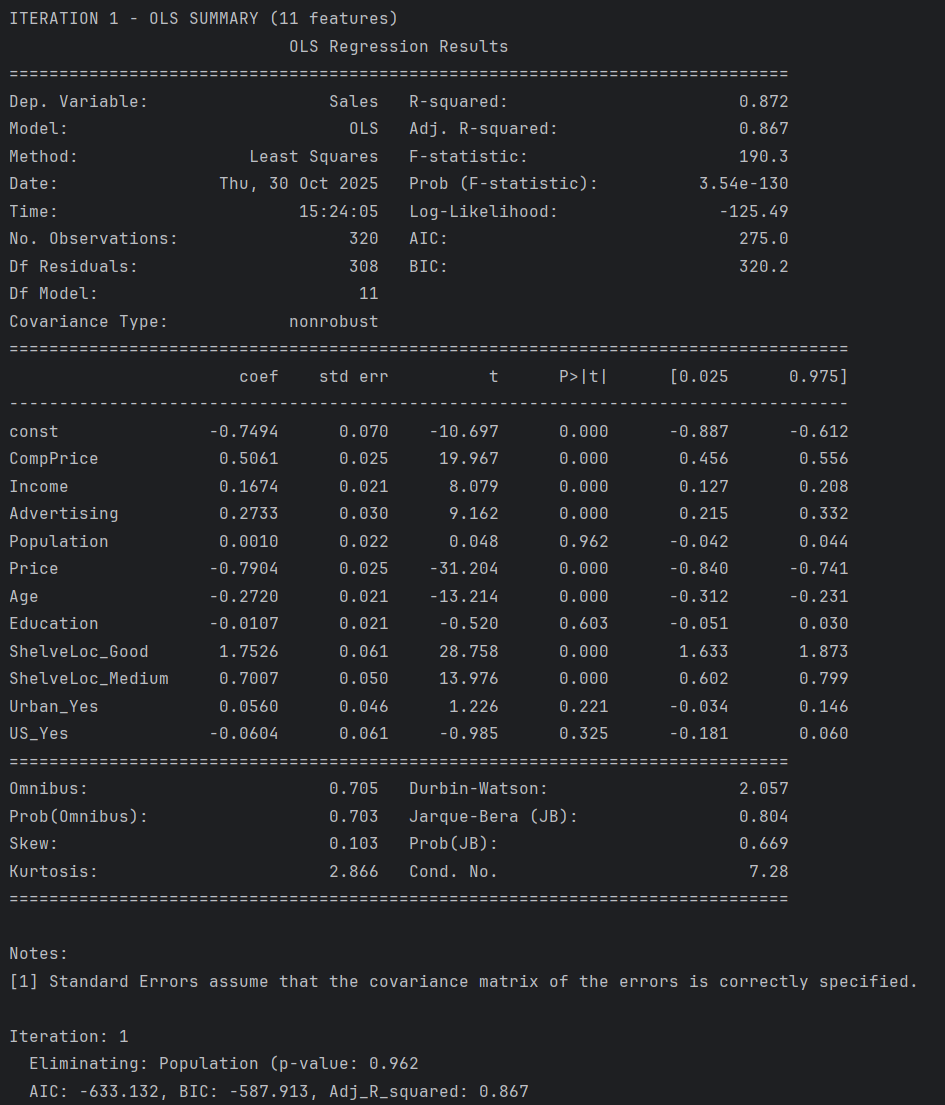
\includegraphics[width=0.85\textwidth]{images/ols_summary_iter1.png}
    \caption{OLS Regression Summary - Iteration 1 (11 features)}
    \label{fig:ols_iter1}
\end{figure}

\begin{figure}[H]
    \centering
    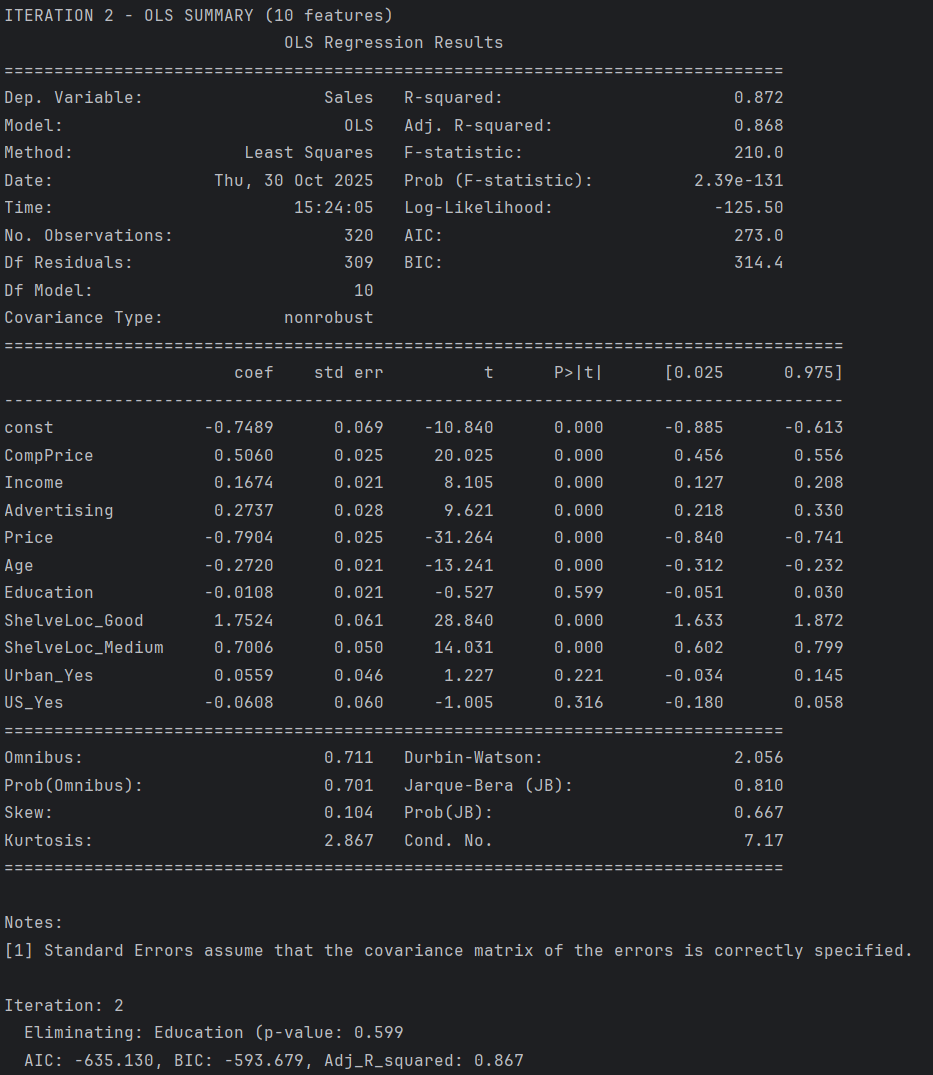
\includegraphics[width=0.85\textwidth]{images/ols_summary_iter2.png}
    \caption{OLS Regression Summary - Iteration 2 (10 features)}
    \label{fig:ols_iter2}
\end{figure}

\begin{figure}[H]
    \centering
    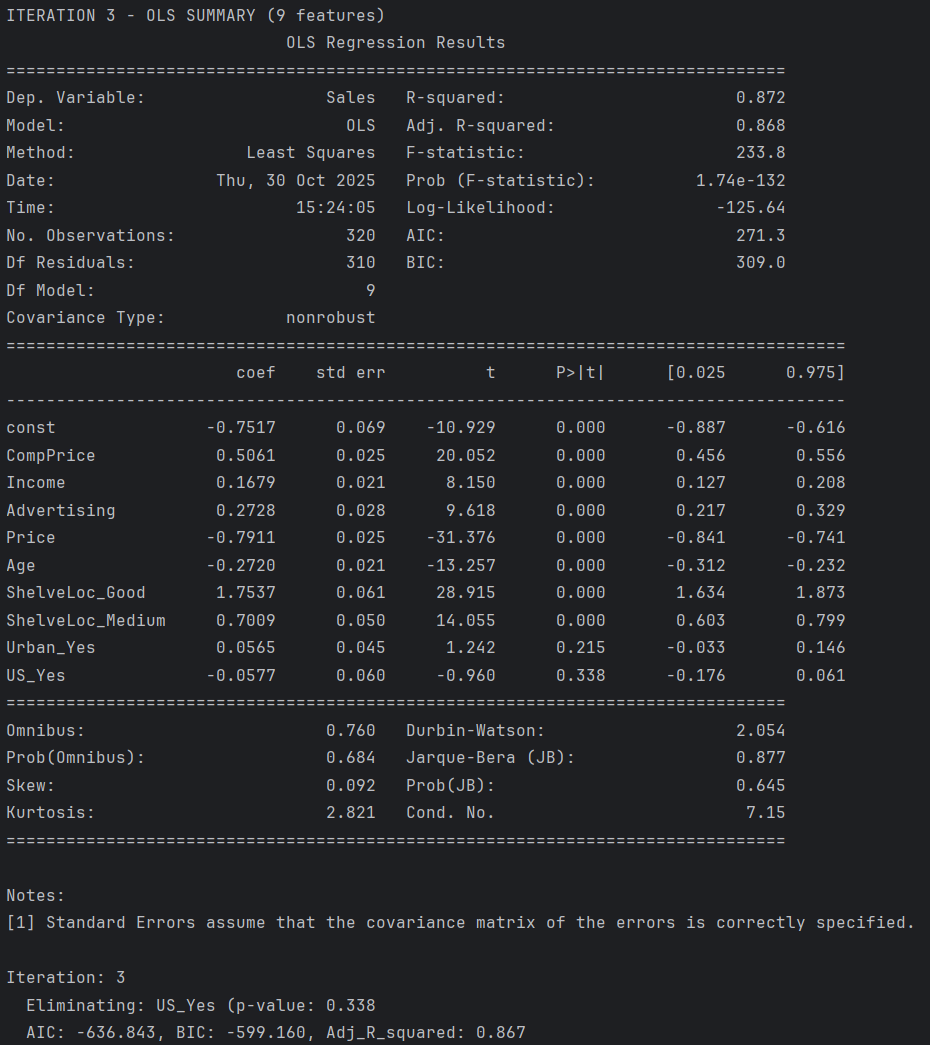
\includegraphics[width=0.85\textwidth]{images/ols_summary_iter3.png}
    \caption{OLS Regression Summary - Iteration 3 (9 features)}
    \label{fig:ols_iter3}
\end{figure}

\begin{figure}[H]
    \centering
    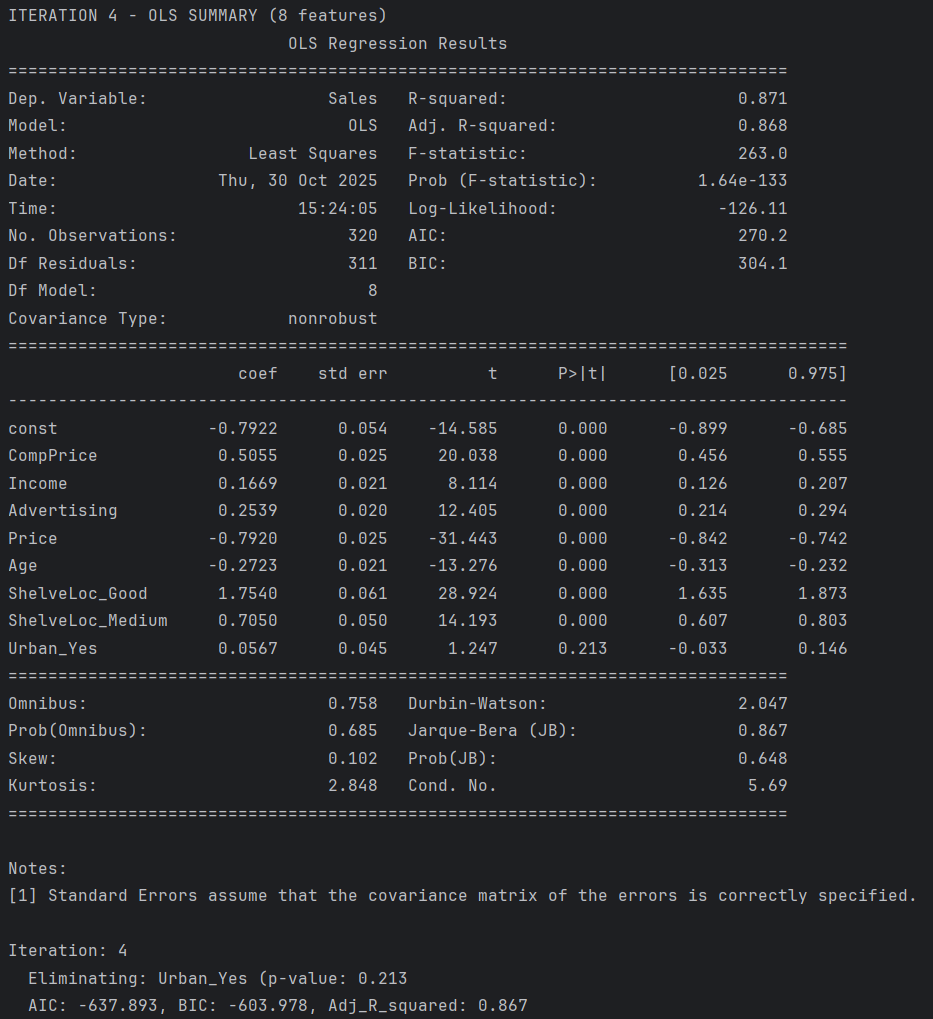
\includegraphics[width=0.85\textwidth]{images/ols_summary_iter4.png}
    \caption{OLS Regression Summary - Iteration 4 (8 features)}
    \label{fig:ols_iter4}
\end{figure}

\begin{figure}[H]
    \centering
    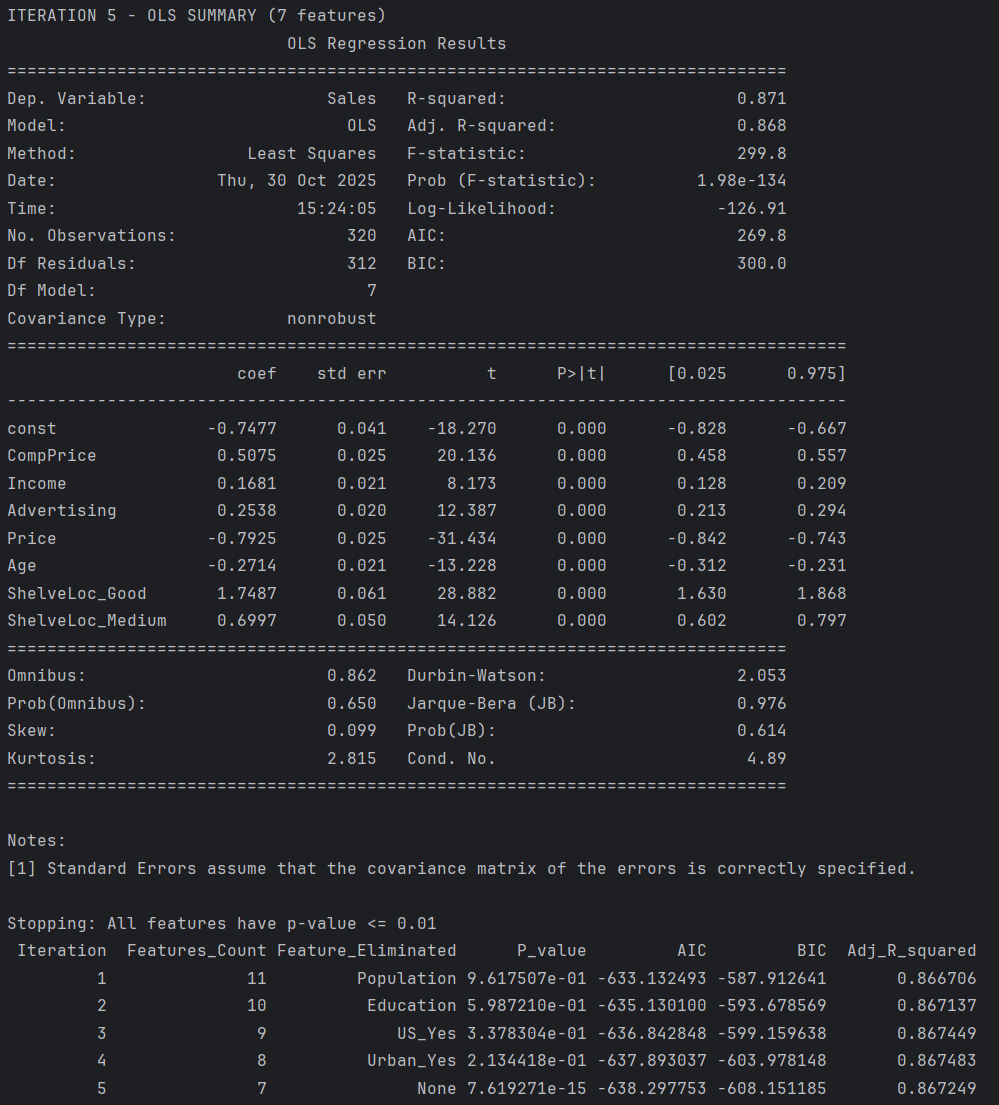
\includegraphics[width=0.85\textwidth]{images/ols_summary_iter5.png}
    \caption{OLS Regression Summary - Iteration 5 (7 features)}
    \label{fig:ols_iter5}
\end{figure}

\textbf{Final Model (Iteration 5) - 7 Features:}
\begin{itemize}
    \item R-squared: 0.871
    \item Adjusted R-squared: 0.868
    \item F-statistic: 299.8
    \item AIC: 269.8
    \item BIC: 300.0
    \item All features have p-value $\leq$ 0.01
\end{itemize}

\subsection{Final Regression Model}

The final regression equation with 7 significant features is:

\begin{equation}
\begin{aligned}
\text{Sales} = &-0.748 + 0.507 \times \text{CompPrice} + 0.168 \times \text{Income} \\
&+ 0.254 \times \text{Advertising} - 0.792 \times \text{Price} \\
&- 0.271 \times \text{Age} + 1.749 \times \text{ShelveLoc\_Good} \\
&+ 0.700 \times \text{ShelveLoc\_Medium}
\end{aligned}
\end{equation}

\subsection{Prediction vs Test Set}


\begin{verbatim}
   Actual_Sales Predicted_Sales Difference
0      2.263812        2.228757   0.035056
1      0.101893       -0.146335   0.248228
2     -0.998528       -0.471935  -0.526593
3     -0.351013       -0.279924  -0.071089
4     -0.602235       -0.469375  -0.132860
5     -0.800381       -1.127828   0.327447
6      0.289424        0.396014  -0.106589
7     -1.391282       -0.397780  -0.993502
8      1.050165        1.321531  -0.271366
9     -0.358090       -0.413283   0.055193
\end{verbatim}


\begin{figure}[H]
    \centering
    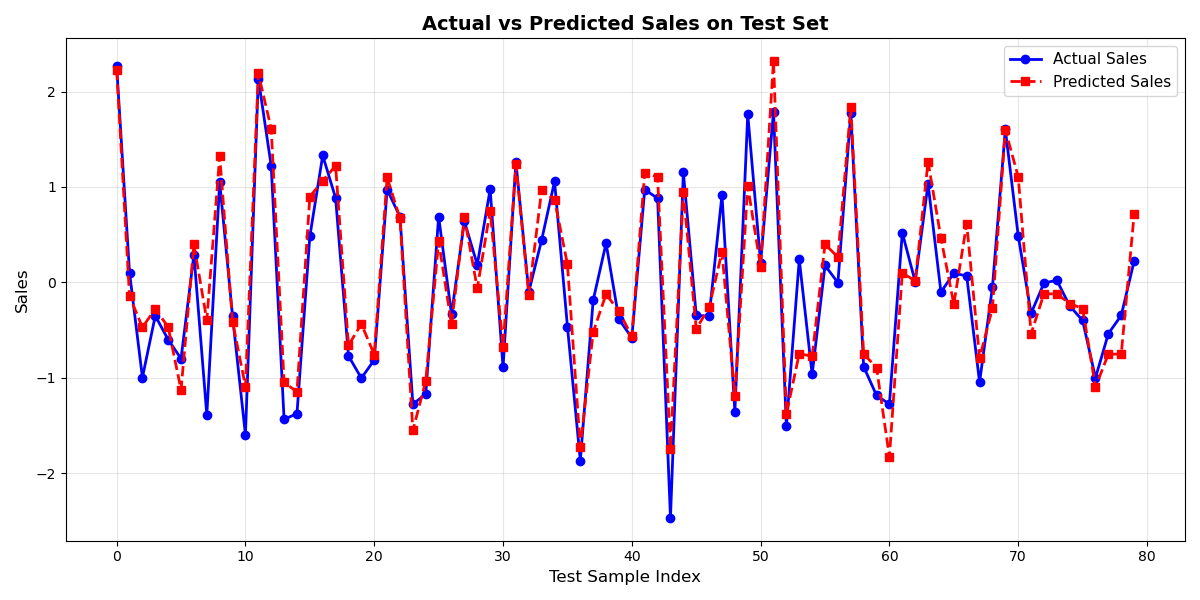
\includegraphics[width=0.7\textwidth]{images/model_performance.png}
    \caption{Original Test Set vs Predicted Sales (Backward Stepwise)}
    \label{fig:stepwise_prediction}
\end{figure}

\subsection{Mean Squared Error}

\begin{itemize}
    \item \textbf{Mean Squared Error (MSE): 0.984}
    \item Root Mean Squared Error (RMSE): 0.992
    \item Mean Absolute Error (MAE): 0.273
\end{itemize}

\section{PCA}

\subsection{95\% Variance Explained}

\textbf{8 principal components} are needed to explain more than 95\% of the variance.

\begin{itemize}
    \item Total number of features: 11
    \item Number of components for 95\% variance: 8
    \item Cumulative variance explained: 0.9512 (95.12\%)
\end{itemize}

\begin{table}[H]
\centering
\caption{Principal Component Analysis - Variance Explained}
\begin{tabular}{ccc}
\toprule
\textbf{Component} & \textbf{Variance Explained} & \textbf{Cumulative Variance} \\
\midrule
PC1 & 0.208 & 0.208 \\
PC2 & 0.172 & 0.381 \\
PC3 & 0.134 & 0.515 \\
PC4 & 0.125 & 0.640 \\
PC5 & 0.122 & 0.762 \\
PC6 & 0.095 & 0.857 \\
PC7 & 0.053 & 0.910 \\
PC8 & 0.042 & \textbf{0.951} \\
PC9 & 0.026 & 0.977 \\
PC10 & 0.013 & 0.990 \\
PC11 & 0.010 & 1.000 \\
\bottomrule
\end{tabular}
\end{table}

\subsection{Cumulative Variance Plot \& 95\% Variance Threshold}

\begin{figure}[H]
    \centering
    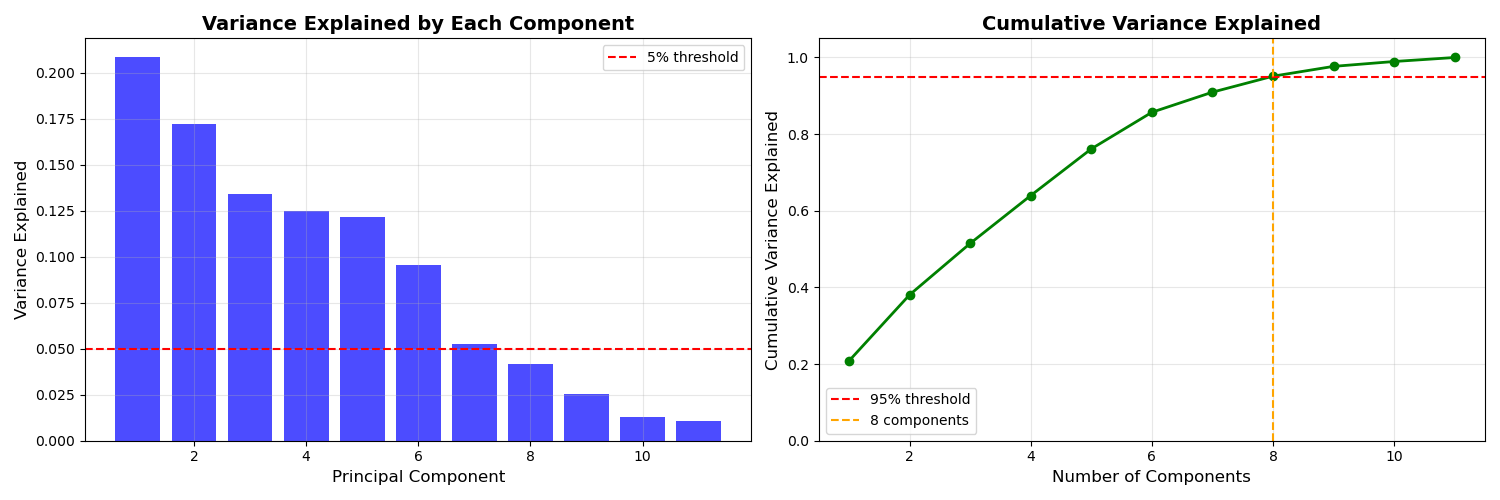
\includegraphics[width=0.9\textwidth]{images/variance_explained.png}
    \caption{Cumulative Explained Variance vs Number of Components \& Horizontal \& Vertical Lines Displaying 95\% Threshold}
    \label{fig:pca_variance}
\end{figure}

\subsection{What Does PCA Say?}
PCA has told us that of the 11 original features, we need 8 principal components to explain 95\% of the variance. This is indicating that our data has some redundancy/correlation,
so after we transform the data into a new coordinate system, we can sufficiently use 8 dimensions instead of 11. However, since PCA gives us a weighted combination of all original features, and not the individual features,
it doesn't tell us explicitly which features to remove, but has created new features for us to use. To learn which features we should remove, we should use backward/forward stepwise regression, or use a Random Forest model to find which features to split on.

\section{Random Forest Analysis}

\subsection{Feature Importance Bar Plot}

The Random Forest analysis identified the following feature importances:

\begin{table}[H]
\centering
\caption{Random Forest Feature Importance}
\begin{tabular}{lc}
\toprule
\textbf{Feature} & \textbf{Importance} \\
\midrule
Price & 0.281 \\
ShelveLoc\_Good & 0.251 \\
CompPrice & 0.108 \\
Age & 0.106 \\
Advertising & 0.066 \\
Income & 0.057 \\
ShelveLoc\_Medium & 0.055 \\
Population & 0.037 \\
Education & 0.029 \\
Urban\_Yes & 0.005 \\
US\_Yes & 0.004 \\
\bottomrule
\end{tabular}
\end{table}

\begin{figure}[H]
    \centering
    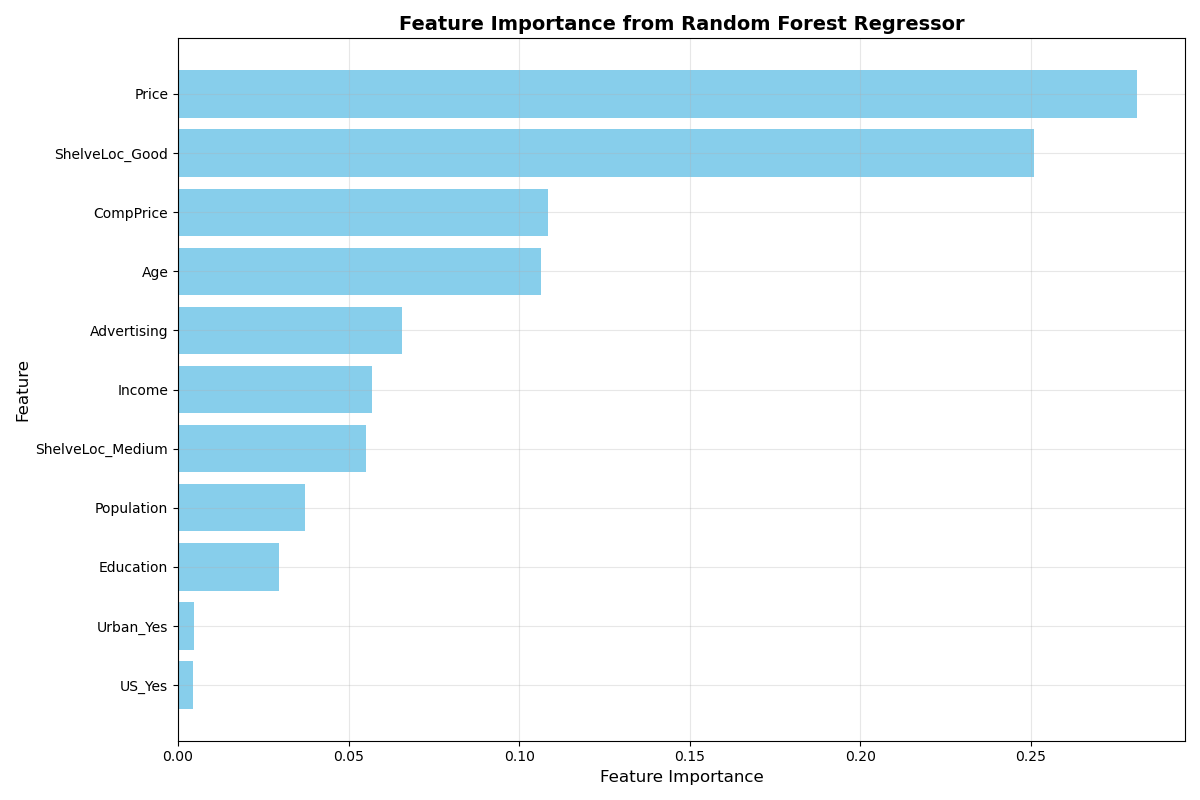
\includegraphics[width=0.7\textwidth]{images/feature_importance.png}
    \caption{Random Forest Feature Importance (Descending Order)}
    \label{fig:rf_importance}
\end{figure}

\subsection{Feature Selection Comparison}

\noindent
\begin{minipage}[t]{0.48\textwidth}
    \textbf{Random Forest Selected Features (7) - Threshold: 0.05:}
    \begin{enumerate}
        \item Price
        \item ShelveLoc\_Good
        \item CompPrice
        \item Age
        \item Advertising
        \item Income
        \item ShelveLoc\_Medium
    \end{enumerate}
\end{minipage}
\hfill
\begin{minipage}[t]{0.48\textwidth}
    \textbf{Random Forest Eliminated Features (4):}
    \begin{enumerate}
        \item Population
        \item Education
        \item Urban\_Yes
        \item US\_Yes
    \end{enumerate}
\end{minipage}

\vspace{0.5cm}

Yes, the selected features from Random Forest and Backward Stepwise Regression are \textbf{identical}. Both methods selected the same 7 features and eliminated the same 4 features (Population, Education, Urban\_Yes, US\_Yes).

\subsection{OLS Regression on Random Forest Selected Features}

The features selected to be remove by Random Forest are the exact same as the features selected by the Backward Stepwise Regression, 
the same as displayed in Figures \ref{fig:ols_iter1} - \ref{fig:ols_iter5}. This means that the OLS summaries are identical. That being
said, I will still include a screenshot!

\begin{figure}[H]
    \centering
    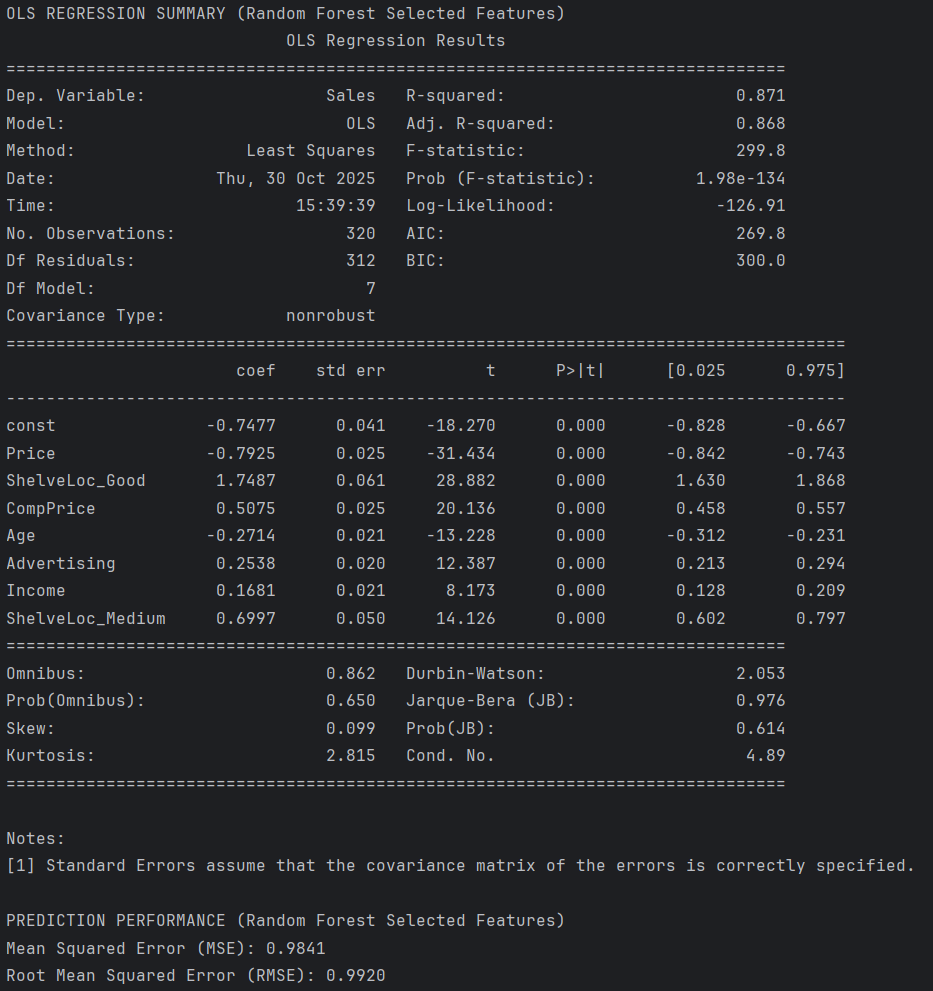
\includegraphics[width=0.8\textwidth]{images/ols_summary_rf.png}
    \caption{OLS Summary (Random Forest Features)}
    \label{fig:rf_ols_summary}
\end{figure}

\subsection{Prediction vs Test Set}

\begin{figure}[H]
    \centering
    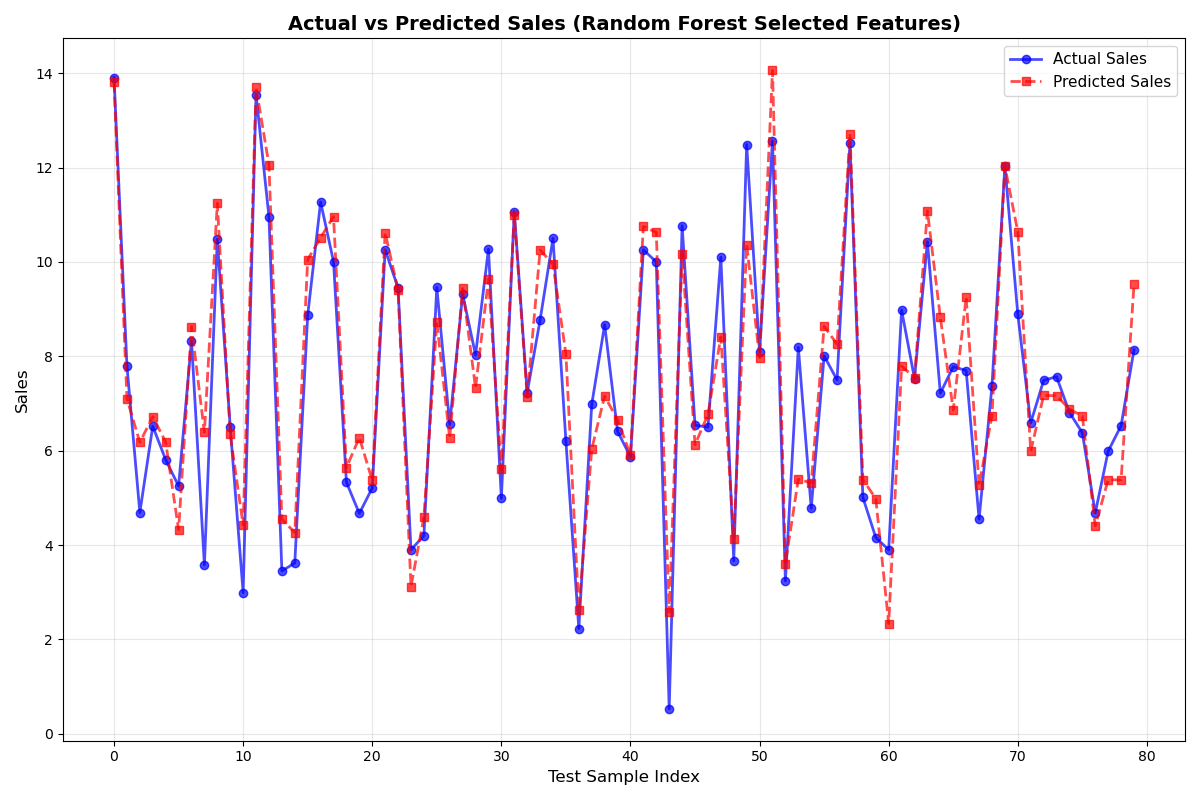
\includegraphics[width=0.7\textwidth]{images/rf_model_performance.png}
    \caption{Original Test Set vs Predicted Sales (Random Forest Features)}
    \label{fig:rf_prediction}
\end{figure}

\subsection{Mean Squared Error}

\begin{itemize}
    \item \textbf{Mean Squared Error (MSE): 0.9841}
    \item Root Mean Squared Error (RMSE): 0.9920
\end{itemize}

\section{Comparison of Feature Selection Methods}

\subsection{Metrics Comparison Table}

There is a \textit{PrettyTable} output in the console of the file, by I have also included a formatted table here.

\begin{table}[H]
\centering
\caption{Model Comparison Summary}
\begin{tabular}{lccccc}
\toprule
\textbf{Model} & \textbf{R²} & \textbf{Adj. R²} & \textbf{AIC} & \textbf{BIC} & \textbf{MSE} \\
\midrule
Backward Stepwise & 0.8706 & 0.8677 & 269.82 & 299.97 & 0.9841 \\
Random Forest & 0.8706 & 0.8677 & 269.82 & 299.97 & 0.9841 \\
\bottomrule
\end{tabular}
\end{table}

\subsection{Recommended Method and Features}

\newpage
Both methods produced \textbf{identical results} in terms of all performance metrics:
\begin{itemize}
    \item Same R² and Adjusted R² (0.8706 and 0.8677)
    \item Same AIC and BIC (269.82 and 299.97)
    \item Same MSE (0.9841)
    \item Same 7 selected features
\end{itemize}

\textbf{Recommended Method:} Either method can be recommended, but:
\begin{itemize}
    \item \textbf{Backward Stepwise Regression} is preferred for interpretability as it provides statistical significance (p-values) for each feature
    \item \textbf{Random Forest} is preferred for capturing non-linear relationships and feature interactions
\end{itemize}

\textbf{Recommended Features for Elimination:}
\begin{enumerate}
    \item Population
    \item Education
    \item Urban\_Yes
    \item US\_Yes
\end{enumerate}

\section{Prediction Interval}

\subsection{95\% Prediction Intervals}

\textbf{Prediction Summary (First 10 rows):}
\begin{table}[H]
\centering
\caption{Prediction Intervals (Standardized Scale)}
\scriptsize
\begin{tabular}{lcccccc}
\toprule
\textbf{Index} & \textbf{Mean} & \textbf{Mean SE} & \textbf{CI Lower} & \textbf{CI Upper} & \textbf{PI Lower} & \textbf{PI Upper} \\
\midrule
18 & 2.229 & 0.075 & 2.081 & 2.376 & 1.497 & 2.961 \\
372 & -0.146 & 0.042 & -0.228 & -0.065 & -0.868 & 0.575 \\
9 & -0.472 & 0.059 & -0.587 & -0.357 & -1.198 & 0.254 \\
127 & -0.280 & 0.033 & -0.345 & -0.215 & -1.000 & 0.440 \\
379 & -0.469 & 0.055 & -0.577 & -0.362 & -1.194 & 0.256 \\
362 & -1.128 & 0.059 & -1.244 & -1.012 & -1.854 & -0.402 \\
26 & 0.396 & 0.069 & 0.260 & 0.532 & -0.334 & 1.126 \\
356 & -0.398 & 0.079 & -0.552 & -0.243 & -1.131 & 0.336 \\
177 & 1.322 & 0.062 & 1.199 & 1.444 & 0.594 & 2.049 \\
131 & -0.413 & 0.047 & -0.506 & -0.321 & -1.136 & 0.310 \\
\bottomrule
\end{tabular}
\end{table}

\textbf{Prediction Intervals (Original Scale - First 10 samples):}
\begin{verbatim}
 Actual_Sales  Predicted_Sales  Lower_95%_PI  Upper_95%_PI  Within_Interval
        13.91         13.810926     11.742477     15.879375             True
         7.80          7.098459      5.059313      9.137605             True
         4.69          6.178252      4.126199      8.230305             True
         6.52          6.720913      4.686524      8.755301             True
         5.81          6.185488      4.136832      8.234144             True
         5.25          4.324572      2.272089      6.377055             True
         8.33          8.631242      6.569331     10.693152             True
         3.58          6.387829      4.315299      8.460358            False
        10.48         11.246932      9.191514     13.302351             True
         6.50          6.344013      4.301129      8.386898             True
\end{verbatim}

\textbf{Coverage Statistics:}
\begin{itemize}
    \item Coverage: 96.250\% of actual values fall within 95\% prediction intervals
    \item Expected: $\sim$95\%
    \item Average prediction interval width: 4.103
\end{itemize}

\subsection{Prediction Interval Plot}

\begin{figure}[H]
    \centering
    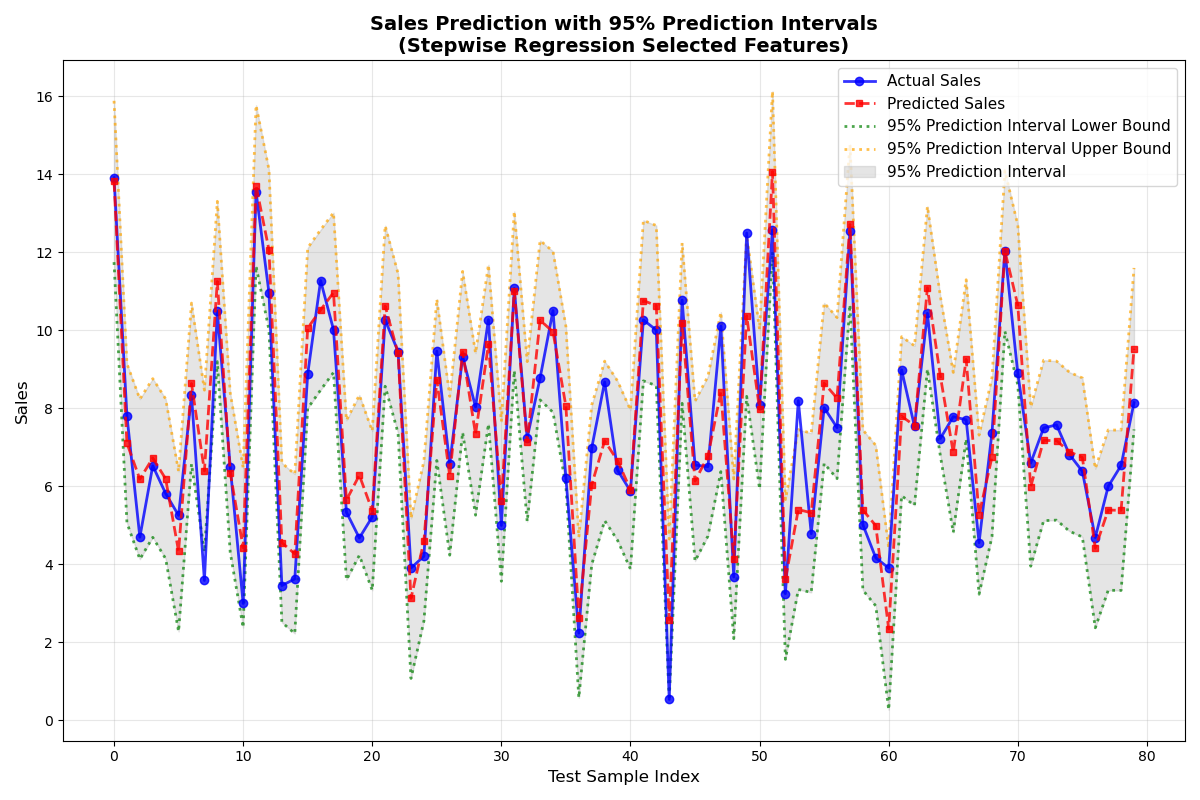
\includegraphics[width=0.8\textwidth]{images/prediction_intervals.png}
    \caption{Predicted Sales with 95\% Prediction Intervals}
    \label{fig:prediction_intervals}
\end{figure}

\newpage
\section{Polynomial Regression and Grid Search}

\subsection{Grid Search with RMSE Minimization}

Grid search was performed with 5-fold cross-validation for polynomial degrees 1 through 15.

\begin{itemize}
    \item Training samples: 320
    \item Testing samples: 80
    \item Cross-validation folds: 5
    \item Total fits: 75 (15 candidates × 5 folds)
\end{itemize}

\subsection{Optimum Polynomial Order}

\boxed{\text{The optimum polynomial degree is n = 4}} with a cross-validation RMSE of 2.565.

\subsection{RMSE vs Polynomial Order Plot}

\begin{table}[H]
\centering
\caption{RMSE for Each Polynomial Degree}
\begin{tabular}{cc}
\toprule
\textbf{Degree} & \textbf{RMSE} \\
\midrule
1 & 2.578 \\
2 & 2.586 \\
3 & 2.574 \\
\textbf{4} & \textbf{2.565} \\
5 & 2.570 \\
6 & 2.577 \\
7 & 2.586 \\
8 & 2.605 \\
9 & 2.646 \\
10 & 2.717 \\
11 & 2.816 \\
12 & 2.939 \\
13 & 3.075 \\
14 & 3.206 \\
15 & 3.312 \\
\bottomrule
\end{tabular}
\end{table}

\begin{figure}[H]
    \centering
    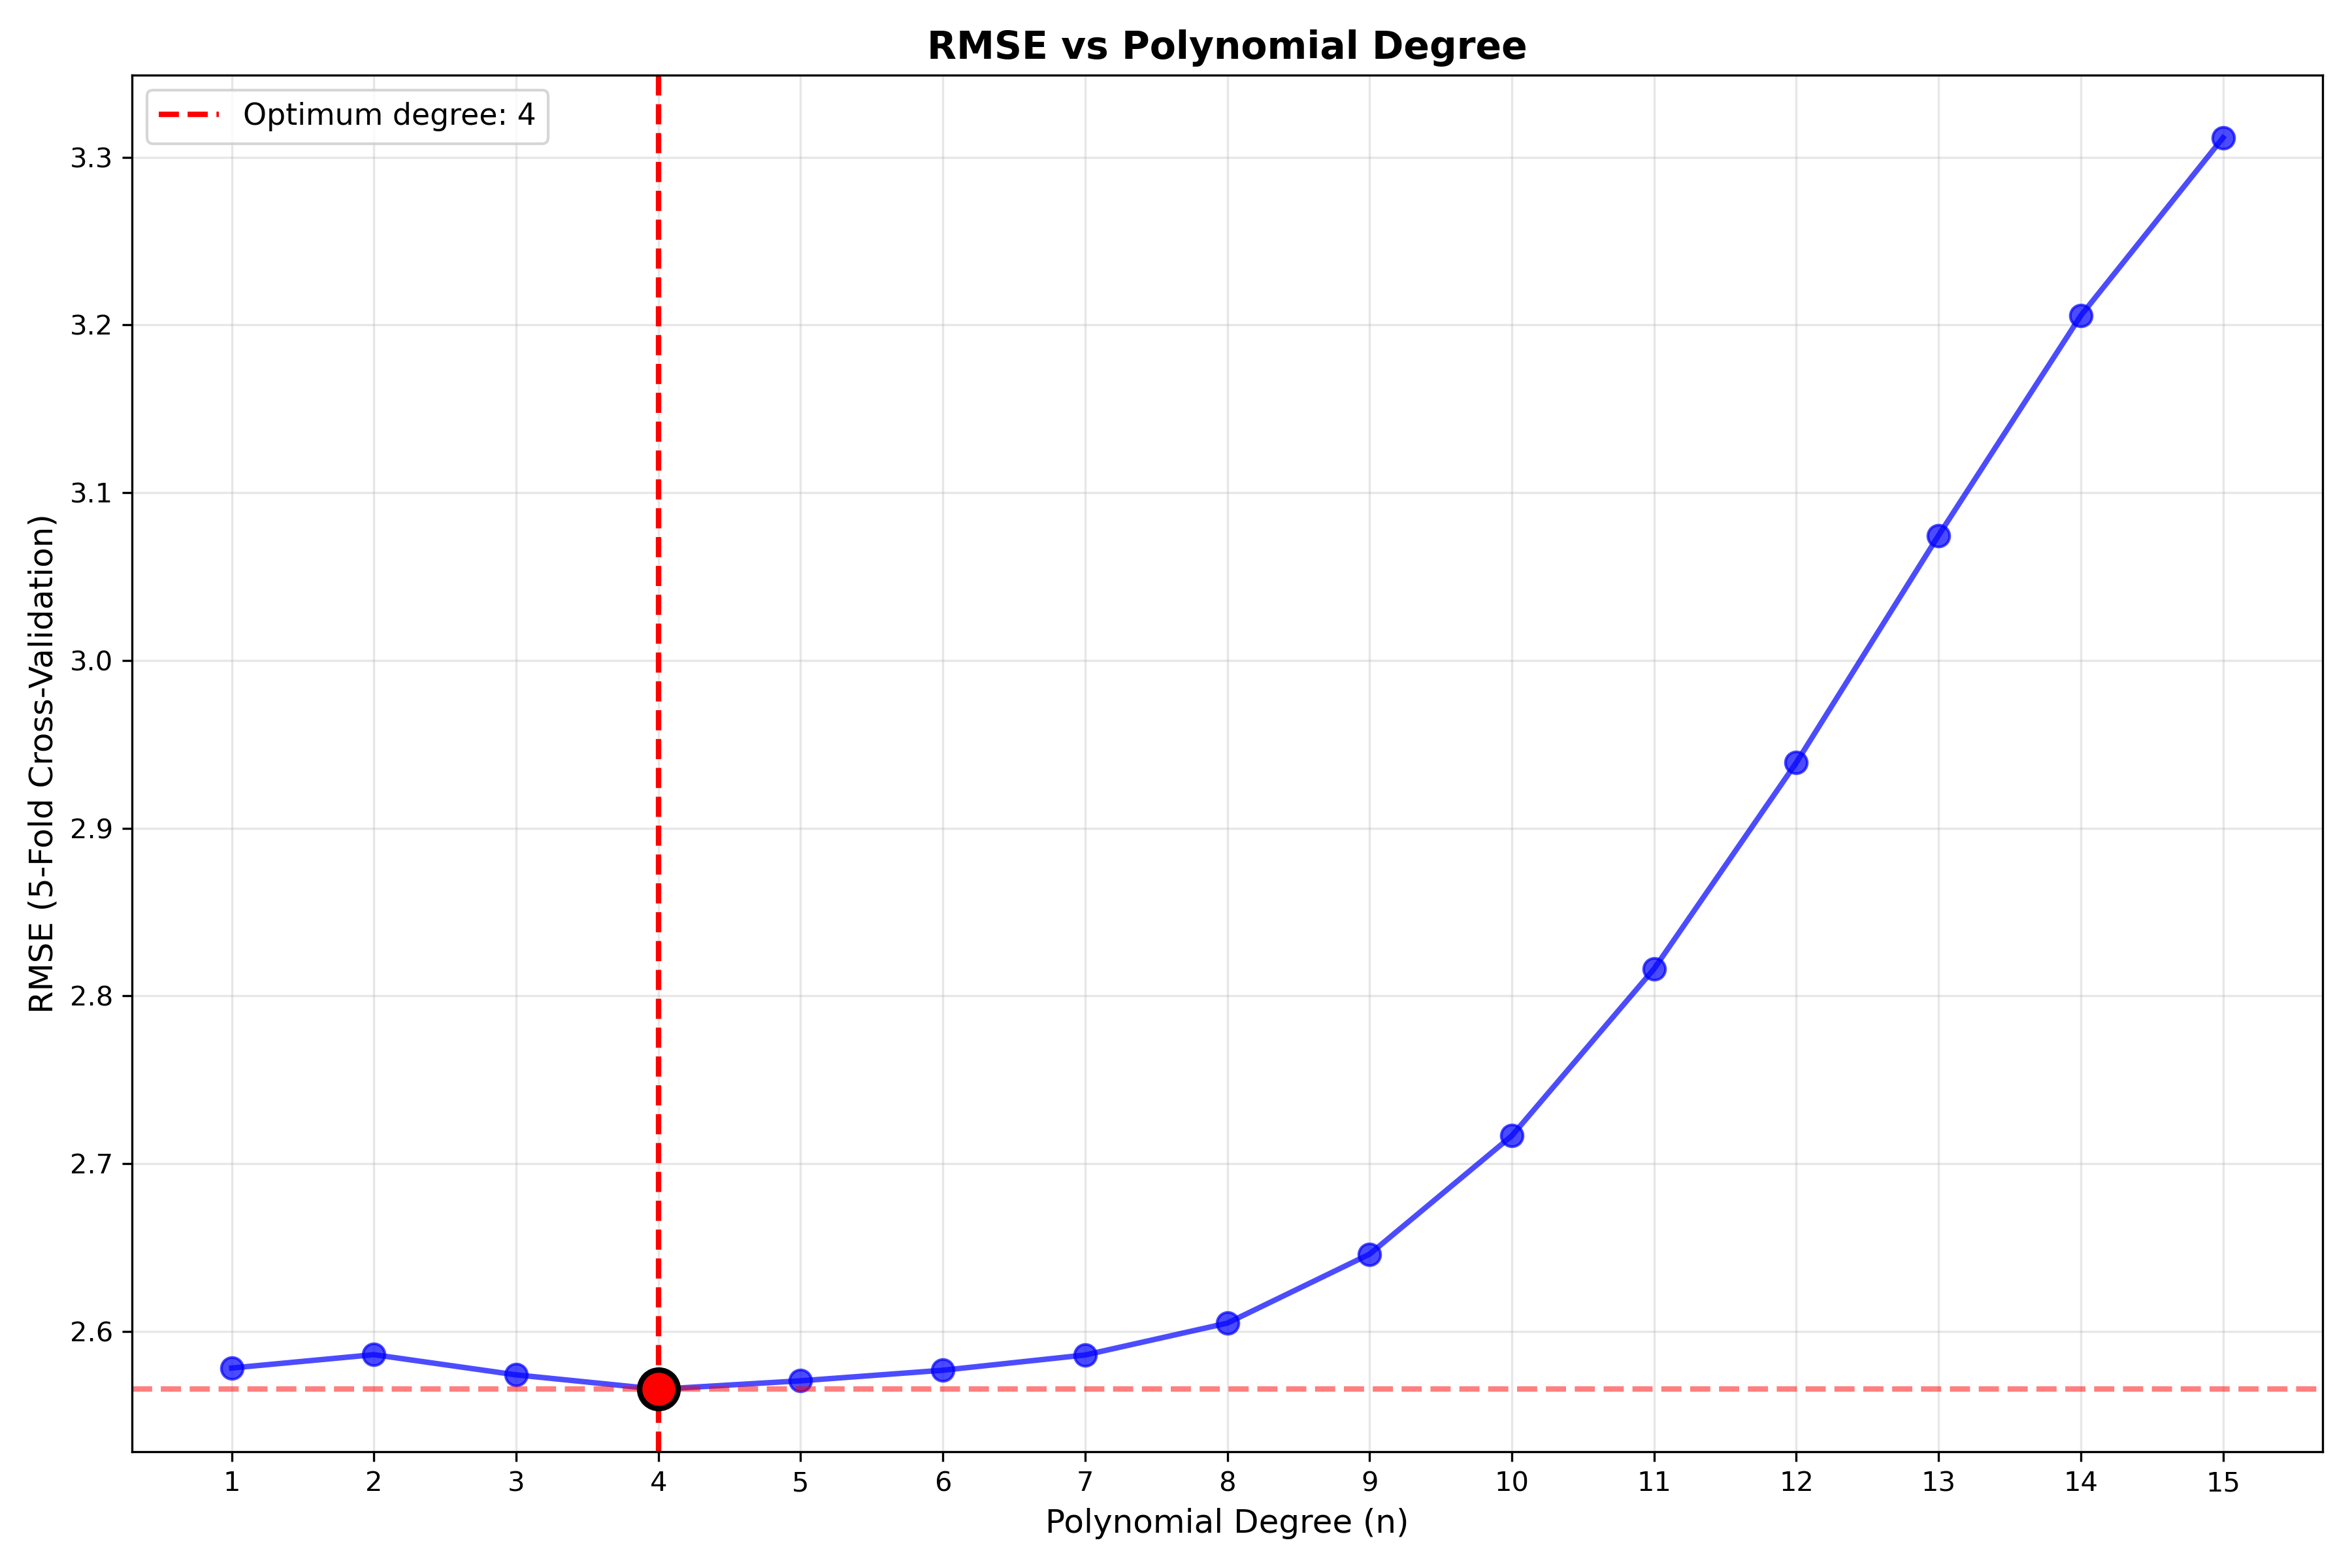
\includegraphics[width=0.8\textwidth]{images/polynomial_degree_rmse.png}
    \caption{RMSE vs Polynomial Degree (n)}
    \label{fig:rmse_polynomial_order}
\end{figure}

\subsection{Training and Prediction}

\begin{figure}[H]
    \centering
    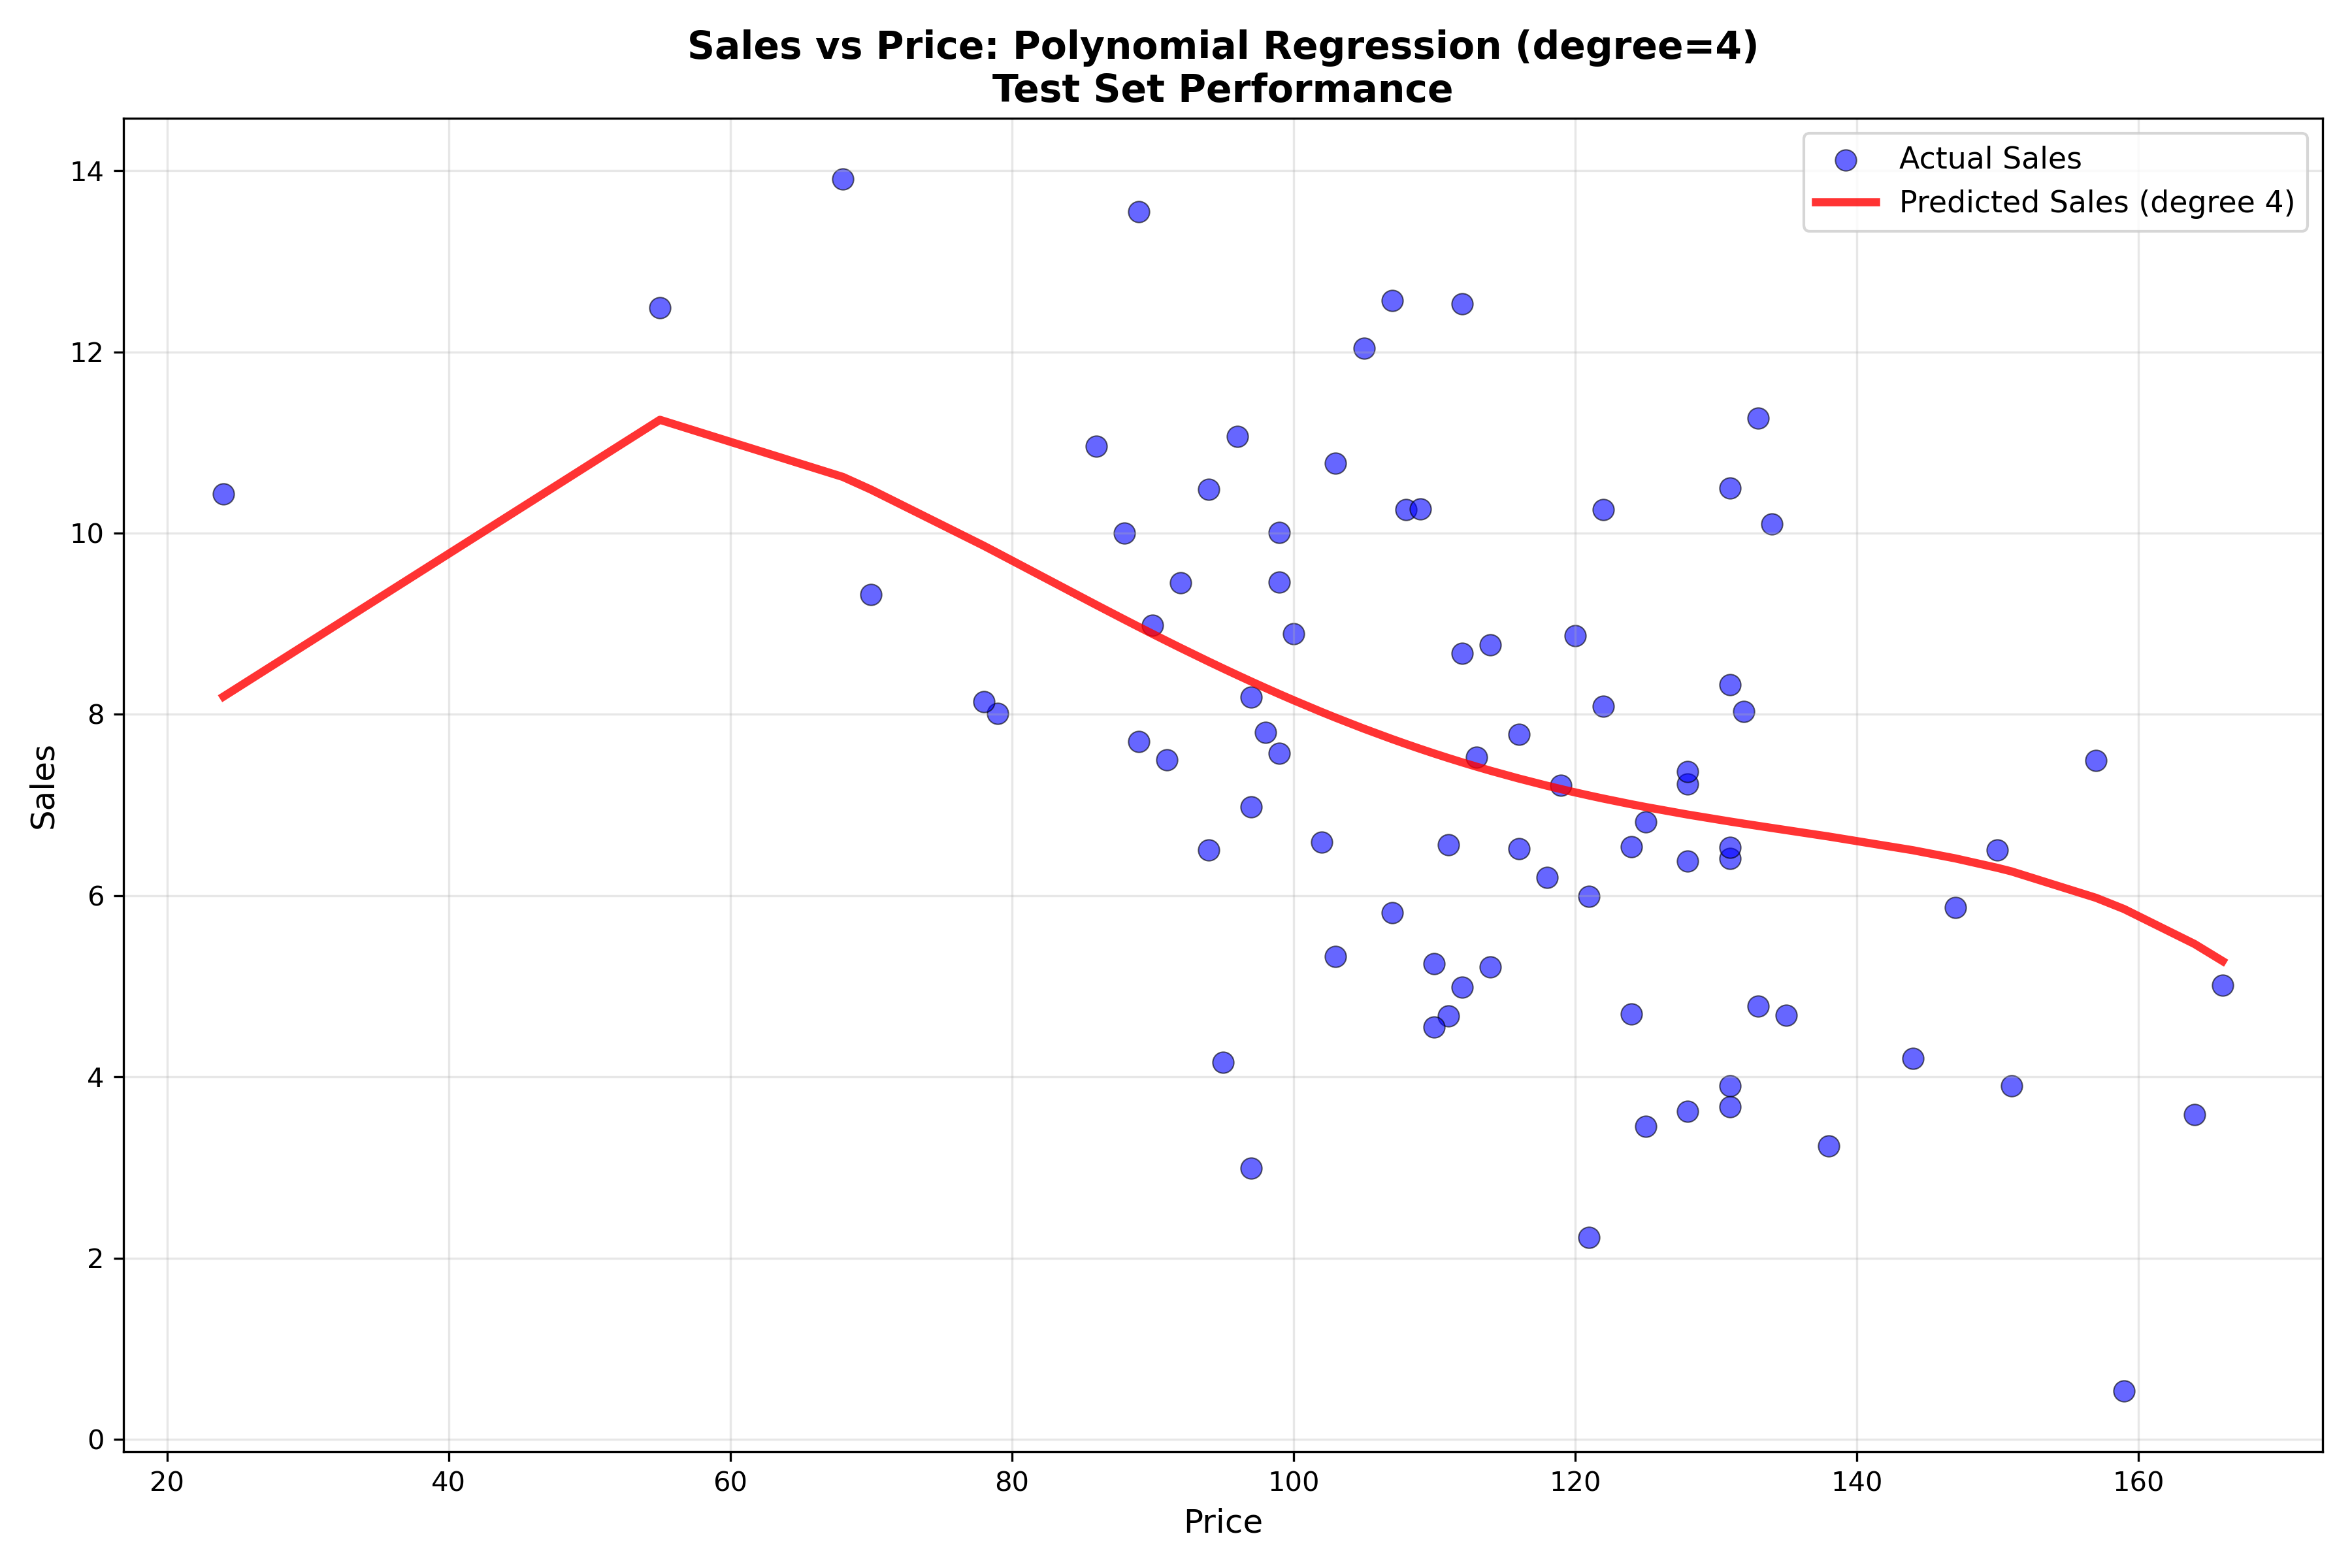
\includegraphics[width=0.7\textwidth]{images/polynomial_prediction.png}
    \caption{Test Set vs Predicted Sales (4th Order Polynomial)}
    \label{fig:poly_prediction}
\end{figure}

\subsection{Mean Squared Error}

\begin{itemize}
    \item Polynomial degree: 4
    \item \textbf{Test Set MSE: 5.826}
    \item Test Set RMSE: 2.414
    \item Test Set R²: 0.255
\end{itemize}

\section{Simple Linear Regression Proof}

In a simple linear regression with n observations:
\begin{equation}
    y_i \approx \hat{\beta}_0 + \hat{\beta}_1 x_i
\end{equation}

Prove the following:
\begin{align}
    \hat{\beta}_1 &= \frac{\sum_{i=1}^{n} (x_i - \bar{x}) (y_i - \bar{y})}{\sum_{i=1}^{n} (x_i - \bar{x})^2} \\
    \hat{\beta}_0 &= \bar{y} - \hat{\beta}_1 \bar{x}
\end{align}

where $\bar{x} = \frac{1}{n} \sum_{i=1}^{n}x_i$ and $\bar{y} = \frac{1}{n}\sum_{i=1}^{n}y_i$ are the sample mean.

First, we have to begin with the Residual Sum of Squares (RSS) equation as given in class:
\begin{equation}
    \text{RSS} = \sum_{i=1}^n (y_i - \hat{\beta}_0 - \hat{\beta}_1 x_i)^2
\end{equation}
and then take the derivative of this equation with respect to $\hat{\beta}_0$ and $\hat{\beta}_1$.

First, we will start with $\hat{\beta}_0$.

\begin{align}
    \frac{\partial \text{RSS}}{\partial \hat{\beta}_0} &= \frac{\partial}{\partial \hat{\beta}_0} \sum_{i=1}^n (y_i - \hat{\beta}_0 - \hat{\beta}_1 x_i)^2 \\
\end{align}

A key part of this derivation is using substitution. We can make $u = y_i - \hat{\beta}_0 - \hat{\beta}_1 x_n$ and then use the
rule $\frac{\partial}{\partial \hat{\beta}_0} u^2 = 2u \frac{\partial u}{\partial \hat{\beta}_0}$. Going from there, we can get
\begin{align}
    \frac{\partial}{\partial \hat{\beta}_0} \sum_{i=1}^n (y_i - \hat{\beta}_0 - \hat{\beta}_1 x_i)^2 &= -2(y_i - \hat{\beta}_0 - \hat{\beta}_1 x_i) \\
    \frac{\partial \text{RSS}}{\partial \hat{\beta}_0} &= \sum_{i=1}^n -2(y_i - \hat{\beta}_0 - \hat{\beta}_1 x_i) \\
\end{align}

Setting the derivation equal to zero, we can continue onward.

\begin{align}
    \frac{\partial \text{RSS}}{\partial \hat{\beta}_0} = -2 \sum_{i=1}^n (y_i - \hat{\beta}_0 - \hat{\beta}_1 x_i) = 0\\
    \sum_{i=1}^n (y_i - \hat{\beta}_0 - \hat{\beta}_1 x_i) = 0 \\
    \sum_{i=1}^n y_i - \sum_{i=1}^n \hat{\beta}_0 - \sum_{i=1}^n \hat{\beta}_1 x_i = 0\\ 
\end{align}

Because $\hat{\beta}_0$ and $\hat{\beta}_1$ are constants, they can come outside the summations. 
For $\hat{\beta}_0$ specifically, the summation will just be $\hat{\beta}_0$ multiplied $n$ times by itself. So, continuing on

\begin{align}
    \sum_{i=1}^n y_i - n \hat{\beta}_0 - \hat{\beta}_1 \sum_{i=1}^n  x_i &= 0\\
    -n \hat{\beta}_0 &= \hat{\beta}_1 \sum_{i=1}^n  x_i - \sum_{i=1}^n y_i\\
    \hat{\beta}_0 &= \frac{1}{n} \sum_{i=1}^n y_i - \hat{\beta}_1 \frac{1}{n} \sum_{i=1}^n  x_i\\ 
\end{align}

Which then becomes
\begin{equation}
    \boxed{\hat{\beta}_0 = \bar{y} - \hat{\beta}_1 \bar{x}}
\end{equation}

Wonderful! Now, to $\hat{\beta}_1$.

\begin{equation}
    \frac{\partial \text{RSS}}{\partial \hat{\beta}_1} = \frac{\partial}{\partial \hat{\beta}_1} \sum_{i=1}^n (y_i - \hat{\beta}_0 - \hat{\beta}_1 x_i)^2
\end{equation}

With the same substitution and rule from the first derivation, we get
\begin{equation}
    \frac{\partial}{\partial \hat{\beta}_1} \sum_{i=1}^n (y_i - \hat{\beta}_0 - \hat{\beta}_1 x_i)^2 = -2x_i (y_i - \hat{\beta}_0 - \hat{\beta}_1 x_i)
\end{equation}

We can then continue on

\begin{align}
    \frac{\partial \text{RSS}}{\partial \hat{\beta}_1} &= -2 \sum_{i=1}^n x_i (y_i - \hat{\beta}_0 - \hat{\beta}_1 x_i) = 0 \\
    \sum_{i=1}^n x_i (y_i - \hat{\beta}_0 - \hat{\beta}_1 x_i) &= 0 \\
    \sum_{i=1}^n x_i (y_i - (\bar{y} - \hat{\beta}_1 \bar{x}) - \hat{\beta}_1 x_i) &= 0 \\
    \sum_{i=1}^n x_i (y_i - \bar{y} - \hat{\beta}_1 (x_i - \bar{x})) &= 0 \\
    \sum_{i=1}^n x_i (y_i - \bar{y}) - \sum_{i=1}^n x_i \hat{\beta}_1 x_i (x_i - \bar{x}) &= 0 \\
    \hat{\beta}_1 &= \frac{\sum_{i=1}^n x_i (y_i - \bar{y})}{\sum_{i=1}^n x_i (x_i - \bar{x})} \\
\end{align}

\end{document}